\chapter{Método propuesto}\label{chapter4}

% **************************** Define Graphics Path **************************
\graphicspath{{Chapter4/Figs/}}

En este capítulo se describe el método propuesto para la integración
de un modelo causal en un algoritmo de aprendizaje por refuerzo para
acelerar su aprendizaje. Primero, se formula el problema a atacar, se delimita
y se describen las suposiciones que se hacen. Además, se presentan algunas definiciones 
importantes para entender el método.
Después, se describe el algoritmo planteado. Finalmente, se muestra como 
ejemplo el problema de los interruptores de luz, una tarea que puede ser atacada
con el marco de trabajo propuesto.

% \begin{itemize}
%     \item \textbf{Descripción del problema y declaración}: Debe 1) presentar
%     el problema de una manera no ambigua, de dos formas, a un alto
%     nivel y a detalle; 2) mostrar por qué el problema es importante,
%     justificar por qué debe ser estudiado. 
%     Describir el problema implicar declarar la meta, los objetivos y delinear las restricciones y suposiciones que han hecho con respecto al problema.
%     \item \textbf{Teoría}: preliminares avanzados, i.e., conocimiento existente que el grupo de lectores puede no estar familiarizado pero es necesario para entender tu solución 
%     \item \textbf{Descripción del método para resolver el problema}:
%      el enfoque y métodos
    
% \end{itemize}
\section{Descripción del problema}

La mayoría de los algoritmos de aprendizaje por refuerzo son métodos genéricos que pueden ser aplicados a cualquier tarea modelada como un proceso de decisión de Markov.
A menudo, estos algoritmos toman bastante tiempo de entrenamiento ya que el agente de RL debe
interactuar a través de prueba y error para explorar su ambiente. 
Sin embargo, en muchas aplicaciones, algunas
propiedades de los problemas pueden ser explotadas para reducir significativamente el tiempo
de entrenamiento del agente. En específico, esta investigación se restringe a hacer frente
a problemas que pueden ser planteados como un proceso de decisión de Markov condicionado a metas
\cite{nair2019causal}. Esto, debido a que de acuerdo  con la definición propuesta por \cite{nair2019causal} este 
tipo de tareas tiene una estructura causal subyacente que describe el comportamiento del ambiente.

    Un MDP condicionado a metas es
una tupla $<\mathcal{S}, \mathcal{A}, \mathcal{X},
\mathcal{D}, \mathcal{P}, \mathcal{G}, r, \gamma, \phi>$, donde 
\begin{itemize}
    \item $\mathcal{S}$ es el espacio de estados, 
    \item $\mathcal{A}$ es el espacio de acciones, 
    \item $\mathcal{X}$ es el conjunto de
    macro-variables de estado \cite{chalupka2014visual} (variables 
    que describen a los estados en un alto nivel), donde $|\mathcal{X}| = N$ y
    $N \ll |S|$,
    \item $\mathcal{D}$ es un grafo causal
    que define relaciones entre
    los conjuntos $\mathcal{A}$ y $\mathcal{X}$, 
    \item $\mathcal{P}: \mathcal{S} \times \mathcal{A} \times \mathcal{S} \rightarrow [0, 1]
     $ es la función de probabilidad de transición de pasar de estado a otro dada una acción. 
    \item $\mathcal{G}$ es el espacio de metas, donde cada uno de sus elementos es un vector $\mathbf{g} = [x_1, \dots, x_N]$ y $x_i \in \mathcal{X}$
    con $i \in \{1, \dots, N\}$,
    \item $r : \mathcal{S} \times \mathcal{A} \times \mathcal{G} \rightarrow \mathbb{R}$ es una función
de recompensa, donde $r(s, a, \mathbf{g})$ produce la recompensa inmediata condicionada a la meta $\mathbf{g} \in \mathcal{G}$,
\item $\gamma$ es el factor de descuento,
\item $\phi : \mathcal{S} \rightarrow \mathcal{X}$ es una función que mapea el espacio de estados al de macro-variables.
\end{itemize}

En un MDP condicionado a metas el objetivo es aprender una 
política óptima condicionada a una meta $\pi^*_g: \mathcal{S} \times \mathcal{G} \rightarrow \mathcal{A}$ que maximice el retorno esperado $R = \sum_{k}^{\infty}\gamma^{k} r(s_k, a_k, g)$.

Un agente de RL que cuente con información adicional que lo vuelva 
capaz de razonar sobre las causas de los cambios en su ambiente 
puede restringir su espacio de búsqueda y
por lo tanto acelerar su entrenamiento.
En concreto, si al agente se le brinda una representación del modelo
causal subyacente de su tarea, esto le permite perseguir acciones que lo lleven a
estados deseados o evitar elegir acciones que lo lleven a 
estados no deseados.

No obstante, definir un modelo causal del ambiente no es una tarea simple.
Las problemas actuales en las que se aplican soluciones 
basadas en RL tienen como características que la información
que recibe el agente normalmente es de alta dimensionalidad, por 
ejemplo, imágenes. Un modelo causal donde se represente toda
la información del ambiente con el que interactúa el agente
es intratable. 
Por lo tanto, se puede aprovechar la propiedad de los MDP condicionado a metas de contar con una
estructura causal $\mathcal{D}$ que describe las relaciones de causa efecto entre las acciones 
y variables de alto nivel que representan lo estados.


\subsection{Suposiciones y limitaciones}

En este trabajo, se consideran  las siguientes suposiciones para limitar el alcance de la solución propuesta.

\begin{enumerate}
    \item El agente conoce el grafo causal $\mathcal{D}$ con todas o
    algunas de las relaciones causales del mundo.
    Por lo tanto,
se puede obtener una especificación precisa de cómo cada variable es influida por sus padres
en la estructura causal $\mathcal{D}$.
%     \item Si se hace una partición del conjunto de variables de la estructura
%     causal en causas y efectos, entonces, en el conjunto de causas están las acciones $\mathcal{A}$ del
% agente, y en el conjunto de consecuencias 
% aquellos pertenecientes a $\mathcal{X}$ que son afectados por una manipulación de una variable de acción.
    \item El espacio de acciones $\mathcal{A}$ es discreto y los valores de las acciones son binarios, $\{0, 1\}$. Esto se puede interpretar como que la acción $a \in \mathcal{A}$ se lleva a cabo o no.
    \item Los elementos de $\mathcal{X}$ son variables con valores binarios, $\{0,1\}$. Esto se puede ver como que la variable $x\in \mathcal{X}$
    está prendida o apagada, es verdadera o falsa o se cumple o no se cumple.
    \item En tareas donde los estados son continuos, el agente de RL cuenta con la función $\phi$ que mapea los estados a variables de alto nivel.
    \item {\color{magenta}Añadir esa suposición de que mis transiciones en estados de alto nivel es inmediata.}
\end{enumerate}


\section{Consultando el modelo causal}

Normalmente, la exploración del agente se lleva a cabo en el paso de la selección de acciones
durante su aprendizaje. Por esta razón,
se propone una variante de la política $\epsilon$-greedy en la que además de las opciones de ejecutar
una acción aleatoria o aquella opción que parece ser mejor hasta ese momento, también se puede elegir consultar el modelo causal. 

Hay dos tipos de consultas que interesa realizar 
sobre la estructura causal: 1)¿qué tal sí hago esta acción?
y 2) ¿qué acción me lleva a cumplir la meta?
La pregunta 1) se puede responder
obteniendo los \textit{sucesores} de la acción $a\in \mathcal{A}$
en el grafo $\mathcal{D}$. Obtener el conjunto de \textit{predecesores} de un efecto $x \in \mathcal{X}$ contesta
a la pregunta 2). Por ahora, este trabajo se limita a hacer consultas del tipo 2), esto es,
simplemente obtener las causas de una variable $x$ para intentar una acción que
sea padre de la variable de interés y evitar aquellas que no sean causa de ésta.

El método propuesto puede trabajar con varios algoritmos
 de RL que utilicen una política $\epsilon$-greedy 
 durante su entrenamiento para elegir sus acciones. En
 este trabajo, se incorpora en el algoritmo Q-learning \cite{watkins1992q}. El proceso de entrenamiento 
 del algoritmo Q-learning se mantiene idéntico salvo por
 la selección de acciones guiada.

El Algoritmo \ref{alg:guided-action-selection} presenta el proceso 
de selección de acciones modificando la política
$\epsilon$-greedy.
El algoritmo recibe como entrada lo siguiente: la estructura causal $\mathcal{D}$, un vector que describe a la meta $\mathbf{g} = [g_1, \dots, g_N]$ donde $g_i \in \mathcal{X}$ y una observación $s \in \mathcal{S}$ del ambiente. La selección de acción se describe a continuación. 

Con probabilidad $1-\epsilon$ se elige la mejor acción. Para el algoritmo Q-learning la mejor acción está dada por aquella acción que da el mayor valor para la función de valor de acción, $\argmax_a Q(s, a)$.
Inicialmente la probabilidad de
explotar la mejor opción es muy baja, es decir, $\epsilon$ inicia con un valor igual o cercano a 1.
Si no se eligió la mejor acción de acuerdo con $Q$, entonces se consulta la estructura causal.

Debido a que la estructura causal está en términos de variables de alto nivel,
entonces, es necesario convertir la observación $s$ a un vector de macro variables $\mathbf{x} = [x_1, \dots, x_N]$, donde $x_i \in \mathcal{X}$. 
Una vez que se
realiza el mapeo entre el espacio de
estados y el de variables de alto nivel se obtiene una lista de variables
de interés, las cuales se consultarán en el grafo causal.
Por simplicidad, esta lista de variables se obtiene calculando
qué variables tiene un valor diferente entre el vector meta $\mathbf{g}$
y el vector de macro variables $\mathbf{x}$.
Sigue el paso de consulta al grafo causal, que consiste en una
obtención de padres de cada variable de interés. Si el grafo causal
logra obtener información sobre alguna de las variables interés, es decir,
ésta se encuentra en el grafo y además tiene al menos un predecesor
se regresa una acción aleatoria que es causa directa de esa variable $x_i$.
En caso de que no se haya información suficiente, la política regresa una acción aleatoria,
es decir, realiza un exploración a ciegas. Para evitar que el orden en que
se obtienen las variables de interés y en el que se obtienen las causas de 
cada variable de interés, se hace un barajado sobre éstas.

\begin{algorithm}[H]
  \caption{Selección de acciones guiada por una estructura causal \label{alg:guided-action-selection}}
  \begin{algorithmic}[1]
  \setstretch{1}
  \REQUIRE Estructura causal $\mathcal{D}$ donde las variables pertenecen a $\mathcal{X} \cup \mathcal{A}$, un vector de variables
  que describe a la meta $\mathbf{g} = [g_1, \dots, g_n]$ donde $g_i \in \mathcal{X}$, una observación del ambiente $s$, probabilidad de exploración $\epsilon$.
  \ENSURE Una acción a ejecutar $a$.
  \STATE Elegir un número aleatorio $r \in [0, 1]$.
  \IF{$r > \epsilon$}
    \RETURN La mejor opción hasta ahora $a$.
   \ENDIF
  \STATE $\mathbf{x} \leftarrow \phi(s)$ \COMMENT{Mapea las observación $s$ a un vector de variables $\mathbf{x} = [x_1, \dots, x_n]$ donde $x_i \in \mathcal{X}$}
   \STATE $E \leftarrow f(\mathbf{g}, \mathbf{x})$ 
  \COMMENT{$f$ Obtiene una lista en orden aleatorio de aquellas variables diferentes $g_i \neq x_i$, donde $g_i, x_i \in \mathcal{X}$}
    \FOR{$e \in E$}
    \IF{$e \in \mathcal{D}$}
        \RETURN Una acción padre de $e$, $a \in \mathcal{A}$ seleccionada aleatoriamente.
    \ENDIF
    \ENDFOR
    \RETURN Acción aleatoria $a$.
  \end{algorithmic}
\end{algorithm}


\section{Ejemplo: Problema de los interruptores de luz}

En esta sección se describe un ejemplo sobre un problema en que se realizan 
lo experimentos de esta investigación. Por ahora, solo se describe el problema
y cómo se aplica el método propuesto.

Imagina que construyes un robot llamado Joi, con el propósito de prender o apagar las luces de las habitaciones 
de una casa de acuerdo a como se le comande.
A Joi se le puede dotar de cierto conocimiento previo de la configuración
del cableado de la casa, tal que le ayude a descifrar las correspondencias entre
interruptores de luz y los focos de las habitaciones. 
 A Joi le gusta aprender mediante prueba
 y error. Además, el robot 
 necesita repetir muchas veces la misma acción para aprender
 qué provocará realizarla. Por lo tanto, si Joi conoce los efectos de algunas de sus acciones (mover los interruptores), puede reducir sus intentos para
 resolver las conexiones entre interruptores y los focos. 
 Por ejemplo, con anticipación Joi puede saber que el mover interruptor de luz $i$ causa que
prenda o apague la luz de la cocina.
 Así que al darle la orden de prender las luces de la cocina, el baño y de alguna otra habitación, Joi solo se enfoca en aprender las partes que no
 conoce.
 
 El problema se puede ver como una tarea donde es necesario tomar las
 decisiones adecuadas para llegar a un configuración de luces deseada. Formalmente, se puede ver como un MDP condicionado a metas donde 
 
 \begin{itemize}
     \item El espacio de estados $\mathcal{S}$, es el conjunto de
     posibles observaciones de la casa desde una vista cenital.
     \begin{figure}[H]
         \centering
         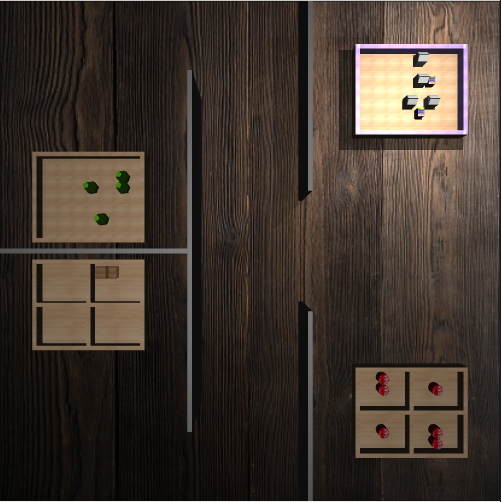
\includegraphics[scale=0.17]{Chapter4/Figs/example_obs.png}
         \caption{Observación disponible para el robot.}
         \label{fig:obs-switches}
     \end{figure}
     \item El espacio de acciones es $\mathcal{A} = \{a_1, a_2, \dots, a_N\}$
     donde cada $a_i$ corresponde a mover o no el interruptor de luz $i$. $a_i = 0$ si no se mueve el interruptor y $a_i = 1$ si se mueve.
     \item El conjunto de variables de alto nivel $\mathcal{X} = \{x_1, x_2, \dots, x_N\}$ contiene
     a las variables que describen el estado de cada foco en la casa. Por ejemplo, $x_i = 1$ establece que el foco $i$ está prendido.
     \item El grafo causal $\mathcal{D} = <\mathcal{A'}, \mathcal{X'}>$, donde
     $\mathcal{A'} \subseteq \mathcal{A}$ y $\mathcal{X'} \subseteq \mathcal{X}$, visualmente el grafo se puede representar de la siguiente forma
     \begin{figure}[H]
         \centering
         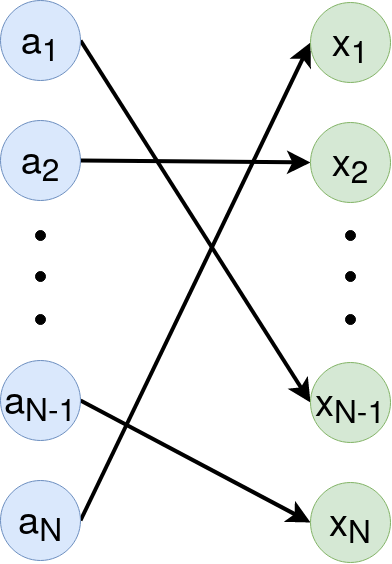
\includegraphics[scale=0.2]{Chapter4/Figs/graph.png}
     \end{figure}
     \item No se cuenta con la función de transición $\mathcal{P}$, sin embargo,
     se conoce que el interruptor $i$ no necesariamente corresponde al foco $i$.
     \item El espacio de metas $\mathcal{G}$ contiene a todas las
     combinaciones posibles de focos prendidos y apagados en la casa.
     \item La recompensa inmediata $r$ se calculas a través de medir de
     una medida de diferencia entre la observación y la meta.
 \end{itemize}
 
 Una vez que la tarea se ha descrito como un MDP, es posible que Joi
 aprenda a alcanzar una configuración de luces deseada
 utilizando un algoritmo de RL, Q-learning por ejemplo. Además,
 dado que suponemos que Joi puede aprovechar el conocimiento que le
 ofrece el grafo causal $\mathcal{D}$, la selección de acciones se puede
 guiar usando el Algoritmo \ref{alg:guided-action-selection}. 
 En la Figura \ref{fig:example-switches} se muestra un paso en el proceso de aprendizaje.
 
 \begin{figure}
     \centering
     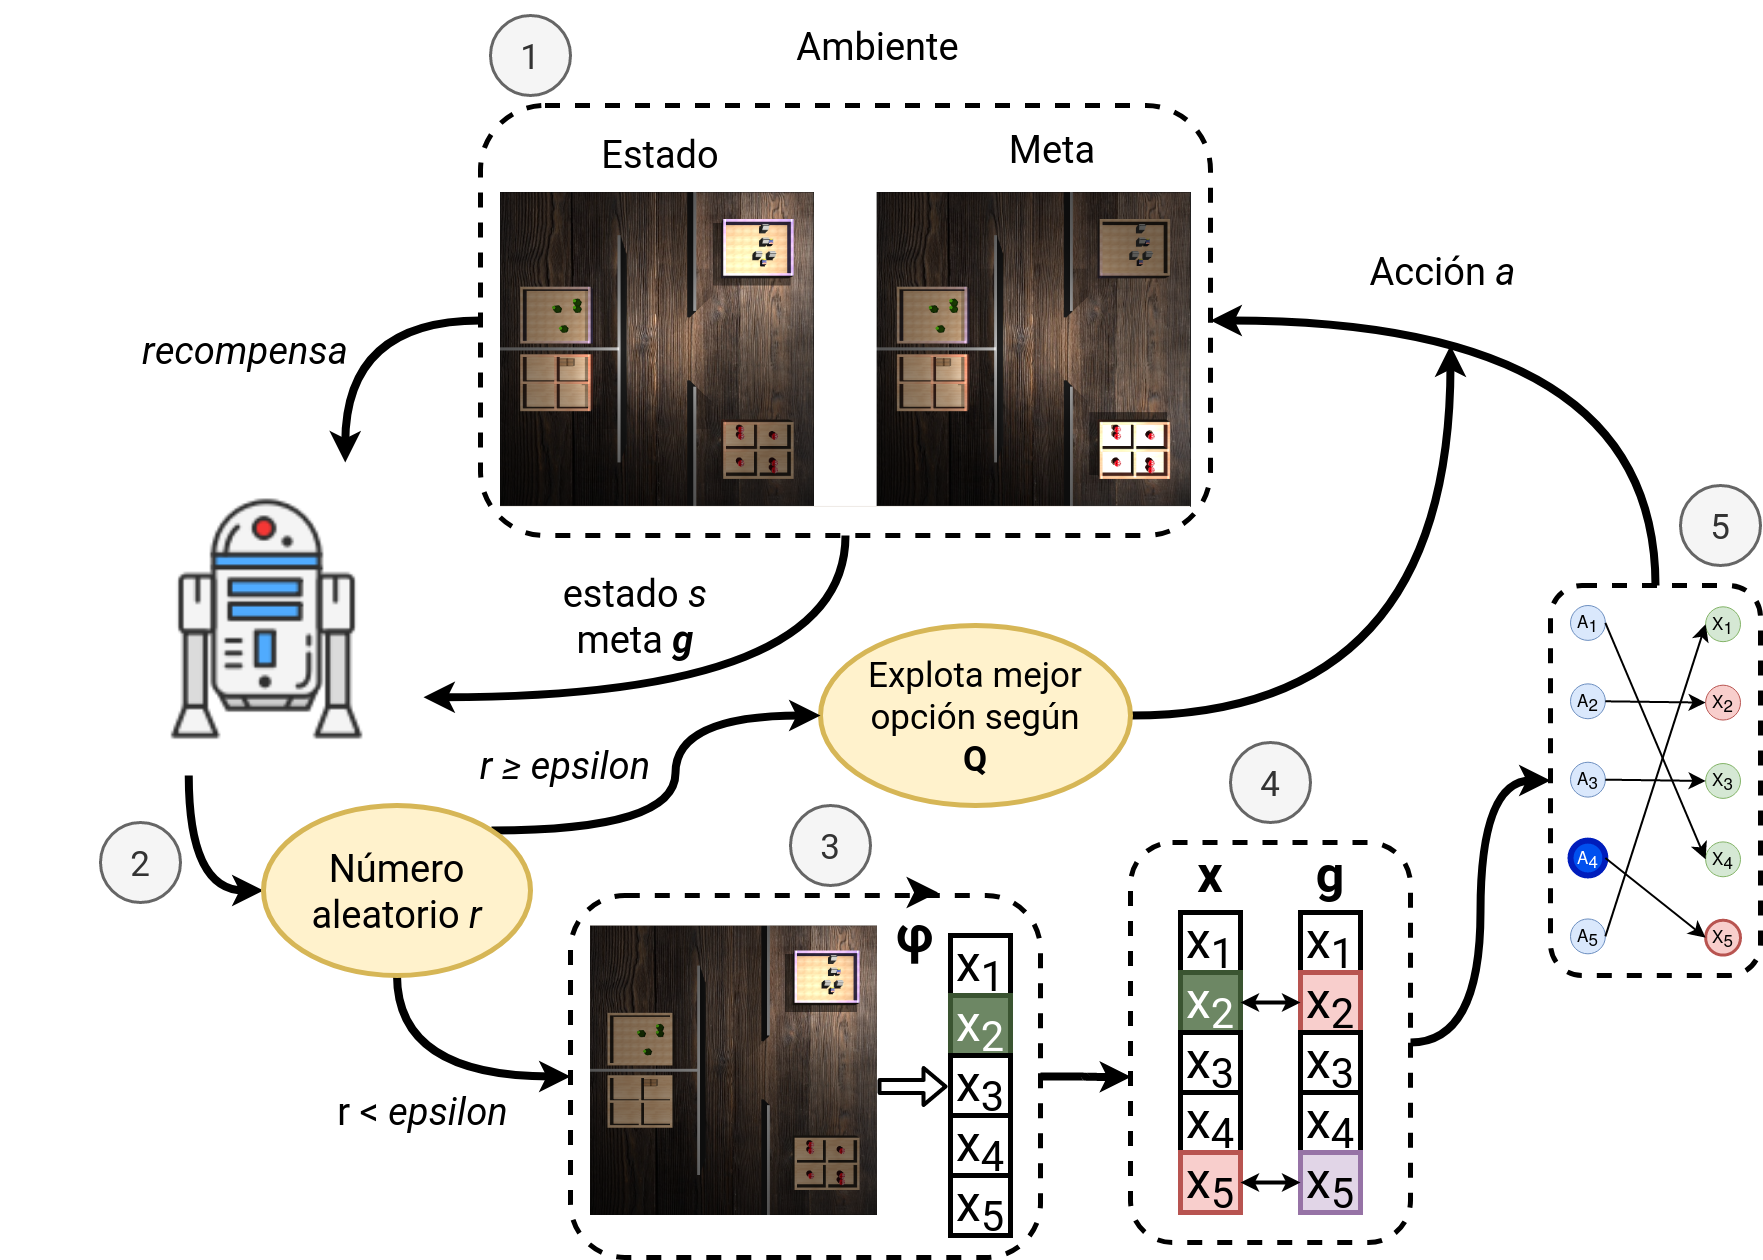
\includegraphics[scale=0.25]{Chapter4/Figs/example_method.png}
     \caption{Interacción del agente con su ambiente: 1) el agente observa el estado de su ambiente además de conocer el vector $\mathbf{g}$, 2) inicia
     la política de selección de acciones, 3) si el agente debe explorar, mapea la observación a un vector de variables de alto nivel $\mathbf{x}$, 4) se calculan los diferentes entre los vectores $\mathbf{x}$ y $\mathbf{g}$, 5) se consultan los padres de las variables de interés y se retorna la acción. El entrenamiento continúa su aprendizaje de manera normal.}
     \label{fig:example-switches}
 \end{figure}